\documentclass[11pt,a4paper]{article}
\usepackage[utf8]{inputenc}
\usepackage[german]{babel}
\usepackage[T1]{fontenc}
\usepackage{amsmath}
\usepackage{amsfonts}
\usepackage{amssymb}
\usepackage{graphicx}
\usepackage[margin=1.25cm]{geometry} % Puts the same margin on all borders of the document

% Packages

\usepackage{hyperref} % Generate hyperlinks to referenced items
\usepackage{adjustbox} % Used to change parameters in \includegraphics[scale=•]{•}
\usepackage{enumitem} % Provides several options for lists
\usepackage{verbatim} % Package to use \begin{comment}
\usepackage{pdfpages} % Used to import PDF pages
\usepackage{multirow} % Allows us to have a single cell in a table span multiple rows
\usepackage{makecell} % Allows us to format multiple lines in a single cell
\usepackage{minted} % Used to syntax highlight code
\usepackage{xcolor}  % Gives access to coloring text
\usepackage{longtable} % Allows us to create a table over multiple pages
\usepackage{float} % Improved placement of floating items
\usepackage{pdfpages} % Used to import pdf pages
\usepackage{booktabs} % Used for horizontal lines instead of \hline



% Settings

\graphicspath{{./files/}} % Sets path for files to the files folder in the same directory

\hypersetup{
    colorlinks=false, %set true if you want colored links
    linktoc=all,     %set to all if you want both sections and subsections linked
    linkcolor=blue,  %choose some color if you want links to stand out
}


\begin{titlepage}
  \title{Rechnerorganisation} % document_name-type_of_document
  \author{Jonas Milkovits}
  \date{Last Edited: \today}
\end{titlepage}

\begin{document}

\pagenumbering{gobble}
\maketitle
\pagenumbering{roman} % i, ii, iii on beginning pages, that don't have content
\tableofcontents
\clearpage
\pagenumbering{arabic} % 1,2,3 on content pages

\section{Einführung}

\subsection{Begrifflichkeiten und Grundlagen}
    \begin{itemize}
        \item \textbf{Abstraktion}
            \begin{itemize}
                \item Wichtiges und zentrales Konzept der Informatik
                \item Verstecken unnötiger Details (für spezielle Aufgabe unnötig)
            \end{itemize}
        
        \item \textbf{Schichtenmodell}
        \item[]
            \begin{minipage}{0.3\textwidth}
            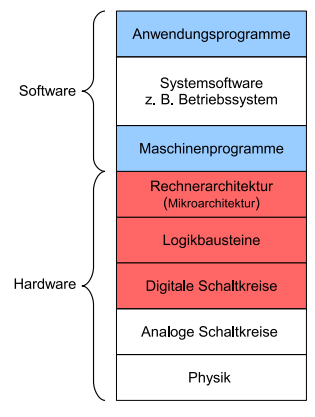
\includegraphics[width=5cm]{schichtenmodell.PNG}
            \end{minipage}
            \begin{minipage}[t]{0.6\textwidth}
            \vspace{-3cm}
                \begin{itemize}
                    \item Untere Schicht erbringt Dienstleistungen für höhere Schicht
                    \item Obere Schicht nutzt Dienste der niedrigeren Schicht
                    \item Eindeutige Schnittstellen zwischen den Schichten
                    \item Vorteile:
                        \begin{itemize}
                            \item Austauschbarkeit einzelner Schichten
                            \item Nur Kenntnis der bearbeitenden Schicht notwendig
                        \end{itemize}
                    \item Nachteile:
                        \begin{itemize}
                            \item ggf. geringere Leistungsfähigkeit des Systems
                        \end{itemize}
                \end{itemize}
            \end{minipage}
        
        \item \textbf{Grundbegriffe}
            \begin{itemize}
                \item Computer:
                    \begin{itemize}
                        \item Datenverarbeitungssystem
                        \item Funktionseinheit zur Verarbeitung und Aufbewahrung von Daten
                        \item Auch Rechner, Informationsverarbeitungssystem, Rechnersystem,..
                        \item Steuerung eines Rechnersystems folgt über ladbares Programm (Maschinenbefehle)
                    \end{itemize}
                \item Grundfunktionen, die ein Rechner ausführt
                    \begin{itemize}
                        \item Verarbeitung von Daten (Rechnen, logische Verknüpfungen,..)
                        \item Speichern von Daten (Ablegen, Wiederauffinden, Löschen)
                        \item Umformen von Daten (Sortieren, Packen, Entpacken)
                        \item Kommunizieren (Mit Benutzer, mit anderen Rechnersystemen)
                    \end{itemize}
            \end{itemize}

        \item \textbf{Komponenten eines Rechnersystems}
            \begin{itemize}
                \item Prozessor
                    \begin{itemize}
                        \item Zentraleinheit, Central Processing Unit (CPU)
                        \item Ausführung von Programmen
                    \end{itemize}
                \item Speicher
                    \begin{itemize}
                        \item Enthält Programme und Daten (Speichersystem)
                    \end{itemize}
                \item Kommunikation
                    \begin{itemize}
                        \item Transfer von Informationen zwischen Speicher und Prozessor
                        \item Kommunikation mit der Außenwelt (Ein-/Ausgabesystem)
                    \end{itemize}
                \item[] 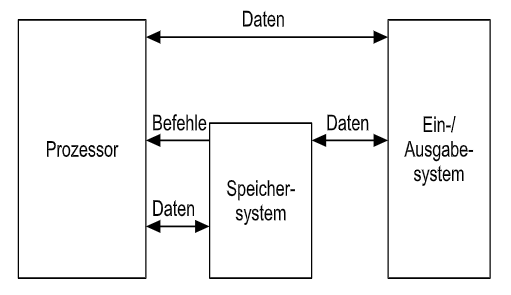
\includegraphics[width=8cm]{rechnersystem.PNG}
            \end{itemize}
    \end{itemize}

\subsection{Streifzug durch die Geschichte}

    \begin{itemize}
        \item \textbf{Übersicht über die geschichtliche Entwicklung mit wichtigsten Meilensteinen}
        \begin{itemize}
            \item[] 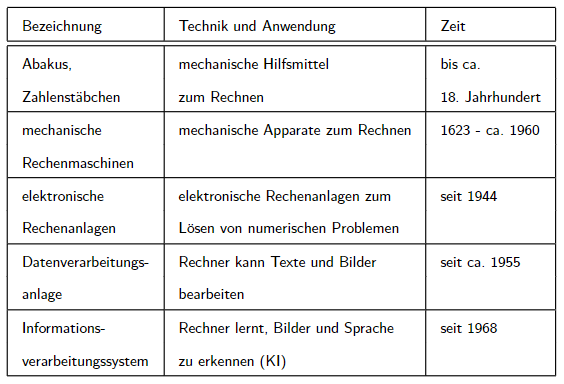
\includegraphics[width=12cm]{geschichtsTabelle1.PNG}
        \end{itemize}
        
        \item \textbf{Fünf Rechnergenerationen im Überblick:}
            \begin{itemize}
                \item[] 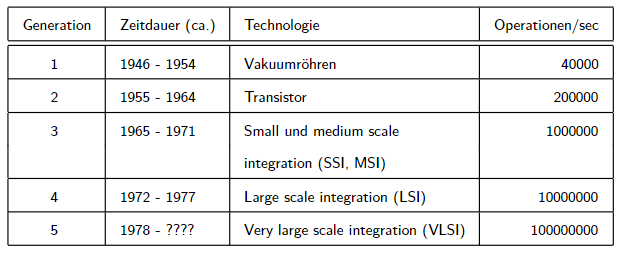
\includegraphics[width=12cm]{rechnergenerationen} 
            \end{itemize}
        
        \item \textbf{Rechner im elektronischen Zeitalter}
            \begin{itemize}
                \item 1954: Entwicklung der Programmiersprache Fortran
                \item 1955: Erster Transistorrechner
                \item 1957: Entwicklung Magnetplattenspeicher, Erste Betriebssysteme für Großrechner
                \item 1968: Erster Taschenrechner
                \item 1971: Erster Mikroprozessor
                \item 1981: Erster IBM PC, Beginn des PC-Zeitalters
            \end{itemize}
    \end{itemize}

\subsection{Ethik in der Informatik}

    \begin{itemize}
        \item Ethik in der Informatik
            \begin{itemize}
                \item Ethik: Bewertung menschlichen Handelns
                \item Verbindung zur Informatik: Anwendung von Rechnern für kriegisches Handelns
                \item \textbf{Dual-Use-Problematik}: Verwendbarkeit von Rechnern für zivile als auch militärische Zwecke
            \end{itemize}
        
        \item Digitale Souveränität
            \begin{itemize}
                \item Souveränität: Fähigkeit zur Selbstbestimmung (Eigenständigkeit, Unabhängigkeit)
                \item Digitale Souveränität: Souveränität im digitalen Raum
            \end{itemize}
    \end{itemize}




\end{document}